\documentclass[aspectratio=169,11pt]{ctexbeamer}
\usetheme{Madrid}
\usecolortheme{dolphin}
\usefonttheme{professionalfonts}
\usepackage{amsmath,amssymb,bm,mathtools}
\usepackage{booktabs,array,multirow}
\usepackage{tikz}
\usetikzlibrary{positioning,arrows.meta,calc,decorations.pathreplacing,fit,shapes.geometric}
\usepackage{pgfplots}
\pgfplotsset{compat=1.18}
\usepackage{algorithmicx}
\usepackage{algpseudocode}
\usepackage{xcolor}
\usepackage{hyperref}

% ---------- Style ----------
\definecolor{MainBlue}{HTML}{174A7E}
\definecolor{DeepBlue}{HTML}{0E2F4F}
\definecolor{AccentOrange}{HTML}{E07A2F}
\definecolor{SoftBlue}{HTML}{EAF2FB}
\definecolor{SoftOrange}{HTML}{FFF0E6}
\definecolor{SoftGreen}{HTML}{EAF7EF}
\definecolor{DarkGreen}{HTML}{1F6F43}
\setbeamercolor{structure}{fg=MainBlue}
\setbeamercolor{title}{fg=white,bg=MainBlue}
\setbeamercolor{frametitle}{fg=white,bg=MainBlue}
\setbeamercolor{block title}{fg=white,bg=MainBlue}
\setbeamercolor{block body}{fg=black,bg=SoftBlue}
\setbeamertemplate{navigation symbols}{}
\setbeamertemplate{itemize item}{\color{AccentOrange}$\blacktriangleright$}
\setbeamertemplate{itemize subitem}{\color{MainBlue}$\circ$}
\setbeamerfont{frametitle}{size=\large,series=\bfseries}
\setbeamerfont{title}{size=\Large,series=\bfseries}
\setbeamertemplate{footline}{%
  \leavevmode%
  \hbox{%
  \begin{beamercolorbox}[wd=.72\paperwidth,ht=2.4ex,dp=1.0ex,leftskip=1.0em]{author in head/foot}%
    \usebeamerfont{author in head/foot}\insertshorttitle
  \end{beamercolorbox}%
  \begin{beamercolorbox}[wd=.28\paperwidth,ht=2.4ex,dp=1.0ex,rightskip=1.0em plus1fil]{date in head/foot}%
    \usebeamerfont{date in head/foot}\insertframenumber{} / \inserttotalframenumber
  \end{beamercolorbox}}%
  \vskip0pt}

% ---------- Commands ----------
\newcommand{\R}{\mathbb{R}}
\newcommand{\C}{\mathbb{C}}
\newcommand{\E}{\mathbb{E}}
\newcommand{\K}{\mathbf{K}}
\newcommand{\I}{\mathbf{I}}
\newcommand{\X}{\mathbf{X}}
\newcommand{\y}{\mathbf{y}}
\newcommand{\alphaVec}{\bm{\alpha}}
\newcommand{\betaVec}{\bm{\beta}}
\newcommand{\PhiMat}{\bm{\Phi}}
\newcommand{\diag}{\operatorname{diag}}
\newcommand{\OO}{\mathcal{O}}
\newcommand{\norm}[1]{\left\lVert #1 \right\rVert}

\title[Frequency-space preconditioning for large-scale KRR]{Frequency-space Preconditioning for Fast Kernel Ridge Regression}
\subtitle{Combining EigenPro-style deflation with Equispaced Fourier Gaussian Processes}
\author{Final Thesis Presentation Draft}
\institute{Your Name \quad | \quad Advisor: \underline{~~~~~~~~}}
\date{\today}

\begin{document}

% 1
\begin{frame}
  \titlepage
  \vspace{-0.4cm}
  \begin{center}
  \small 30-minute presentation structure: problem $\rightarrow$ bottleneck $\rightarrow$ two existing ideas $\rightarrow$ proposed algorithm $\rightarrow$ experiments.
  \end{center}
\end{frame}

% 2
\begin{frame}{One-slide summary}
\begin{columns}[T,onlytextwidth]
\column{0.48\textwidth}
\begin{block}{Problem}
Kernel ridge regression is statistically attractive, but naive solvers require dense kernel matrices.
\[
  (\K + \lambda \I)\alphaVec = \y,
  \qquad \K_{ij}=k(x_i,x_j).
\]
For very large $N$, both storage and iterations are the bottleneck.
\end{block}
\column{0.48\textwidth}
\begin{block}{Thesis idea}
For translation-invariant kernels in low dimension, EFGP turns KRR into a Fourier-space linear system with FFT/NUFFT acceleration. My work adds an EigenPro-style deflation preconditioner in this frequency space.
\end{block}
\end{columns}
\vspace{0.25cm}
\begin{center}
\tikz[baseline]{\node[rounded corners,fill=SoftOrange,draw=AccentOrange,inner sep=6pt,text width=.90\linewidth,align=center]{\large Target: reduce total cost from repeated $\OO(N^2)$ kernel work toward $\OO(N\log N)$-style scaling.};}
\end{center}
\end{frame}

% 3
\begin{frame}{Talk roadmap}
\begin{center}
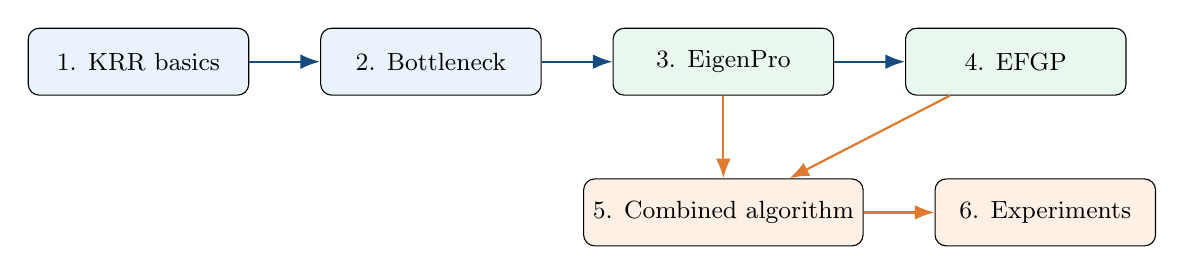
\begin{tikzpicture}[node distance=0.9cm, every node/.style={font=\small}]
\node[draw,rounded corners,fill=SoftBlue,minimum width=2.8cm,minimum height=0.85cm] (a) {1. KRR basics};
\node[draw,rounded corners,fill=SoftBlue,minimum width=2.8cm,minimum height=0.85cm,right=of a] (b) {2. Bottleneck};
\node[draw,rounded corners,fill=SoftGreen,minimum width=2.8cm,minimum height=0.85cm,right=of b] (c) {3. EigenPro};
\node[draw,rounded corners,fill=SoftGreen,minimum width=2.8cm,minimum height=0.85cm,right=of c] (d) {4. EFGP};
\node[draw,rounded corners,fill=SoftOrange,minimum width=2.8cm,minimum height=0.85cm,below=1.05cm of c] (e) {5. Combined algorithm};
\node[draw,rounded corners,fill=SoftOrange,minimum width=2.8cm,minimum height=0.85cm,right=of e] (f) {6. Experiments};
\draw[-{Latex[length=2.5mm]},thick,MainBlue] (a) -- (b);
\draw[-{Latex[length=2.5mm]},thick,MainBlue] (b) -- (c);
\draw[-{Latex[length=2.5mm]},thick,MainBlue] (c) -- (d);
\draw[-{Latex[length=2.5mm]},thick,AccentOrange] (c) -- (e);
\draw[-{Latex[length=2.5mm]},thick,AccentOrange] (d) -- (e);
\draw[-{Latex[length=2.5mm]},thick,AccentOrange] (e) -- (f);
\end{tikzpicture}
\end{center}
\vspace{0.2cm}
\small
The story is not “invent a new kernel”; it is “make the same useful kernel model solvable at a much larger scale.”
\end{frame}

\section{Motivation and KRR fundamentals}

% 4
\begin{frame}{Why kernel ridge regression still matters}
\begin{columns}[T,onlytextwidth]
\column{0.58\textwidth}
\begin{itemize}
  \item \textbf{Strong statistical theory}: RKHS regularization, representer theorem, minimax results for Sobolev-type spaces.
  \item \textbf{Stable optimization}: convex objective, no architectural search or nonconvex training dynamics.
  \item \textbf{Competitive regimes}: small/medium data, tabular data, scientific regression, spatial statistics.
  \item \textbf{Modern relevance}: wide neural networks induce kernels; recent Fourier/NUFFT work shows kernels can be extremely scalable in structured settings.
\end{itemize}
\column{0.38\textwidth}
\begin{block}{Regularized risk}
\[
\min_{f\in\mathcal{H}_k}
\frac{1}{N}\sum_{i=1}^{N}(f(x_i)-y_i)^2 + \lambda \norm{f}_{\mathcal{H}_k}^2.
\]
\end{block}
\begin{block}{Representer theorem}
\[
 f(x)=\sum_{i=1}^{N}\alpha_i k(x,x_i).
\]
\end{block}
\end{columns}
\vspace{0.1cm}
\tiny Sources: Bach, \emph{Learning Theory from First Principles}; Doum\`eche et al., 2025; Abedsoltan et al., 2023.
\end{frame}

% 5
\begin{frame}{KRR fundamentals: from function space to a linear system}
\begin{columns}[T,onlytextwidth]
\column{0.48\textwidth}
\begin{block}{Training problem}
Given $\{(x_i,y_i)\}_{i=1}^{N}$ and kernel $k$, solve
\[
\min_{\alphaVec\in\R^N}
\norm{\K \alphaVec-\y}^2 + \lambda\alphaVec^T\K\alphaVec.
\]
First-order condition gives
\[
(\K+\lambda\I)\alphaVec=\y.
\]
\end{block}
\column{0.48\textwidth}
\begin{block}{Prediction}
\[
\widehat f(x)=k(x,X)^T\alphaVec.
\]
Equivalent to GP posterior mean when $\lambda=\sigma^2$.
\end{block}
\begin{block}{Core numerical object}
\[
A\alphaVec = \y,\qquad A=\K+\lambda\I.
\]
All scalability questions become: how fast can we apply or solve with $A$?
\end{block}
\end{columns}
\end{frame}

% 6
\begin{frame}{Computational bottleneck: dense kernel matrices}
\begin{columns}[T,onlytextwidth]
\column{0.50\textwidth}
\begin{block}{Direct method}
\begin{itemize}
  \item Form $\K$: $\OO(N^2)$ kernel evaluations.
  \item Store $\K$: $\OO(N^2)$ memory.
  \item Cholesky solve: $\OO(N^3)$ time.
\end{itemize}
\end{block}
\begin{block}{Iterative method}
\begin{itemize}
  \item CG only needs matrix-vector products.
  \item But dense $\K v$ is still $\OO(N^2)$ per iteration.
  \item Bad conditioning can make iteration count large.
\end{itemize}
\end{block}
\column{0.45\textwidth}
\begin{center}
\begin{tabular}{rcc}
\toprule
$N$ & entries in $\K$ & double memory \\
\midrule
$10^4$ & $10^8$ & 0.8 GB \\
$10^5$ & $10^{10}$ & 80 GB \\
$10^6$ & $10^{12}$ & 8 TB \\
\bottomrule
\end{tabular}
\end{center}
\vspace{0.35cm}
\begin{center}
\tikz[baseline]{\node[fill=SoftOrange,draw=AccentOrange,rounded corners,inner sep=5pt]{The matrix is the model - and also the bottleneck.};}
\end{center}
\end{columns}
\end{frame}

% 7
\begin{frame}{Iterative method: Conjugate Gradient and conditioning}
\begin{columns}[T,onlytextwidth]
\column{0.53\textwidth}
\begin{block}{CG for SPD systems}
For $A=\K+\lambda\I \succ 0$:
\[
\alpha_{t+1}\in\alpha_0 + \mathcal{K}_{t}(A,r_0),\quad
\mathcal{K}_{t}=\operatorname{span}\{r_0,Ar_0,\ldots,A^{t-1}r_0\}.
\]
\end{block}
\begin{block}{Classical convergence proxy}
\[
\frac{\norm{e_t}_{A}}{\norm{e_0}_{A}}
\leq
2\left(\frac{\sqrt{\kappa(A)}-1}{\sqrt{\kappa(A)}+1}\right)^t.
\]
\end{block}
\column{0.42\textwidth}
\begin{center}
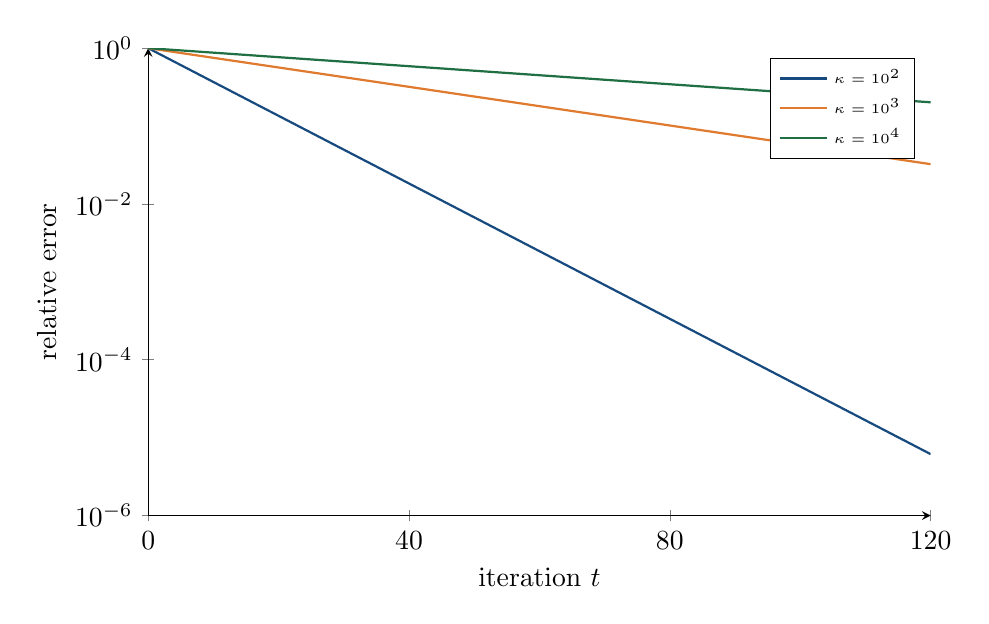
\begin{tikzpicture}
\begin{axis}[
width=0.95\linewidth,height=0.62\linewidth,
axis lines=left,xlabel={iteration $t$},ylabel={relative error},
ymode=log, xmin=0,xmax=120,ymin=1e-6,ymax=1,
legend style={font=\tiny,at={(0.98,0.98)},anchor=north east},
xtick={0,40,80,120},ytick={1,1e-2,1e-4,1e-6}]
\addplot[MainBlue,thick,domain=0:120,samples=100]{exp(-x/10)};
\addlegendentry{$\kappa=10^2$}
\addplot[AccentOrange,thick,domain=0:120,samples=100]{exp(-x/35)};
\addlegendentry{$\kappa=10^3$}
\addplot[DarkGreen,thick,domain=0:120,samples=100]{exp(-x/75)};
\addlegendentry{$\kappa=10^4$}
\end{axis}
\end{tikzpicture}
\end{center}
\small
Bad spectrum means either more iterations or a preconditioner.
\end{columns}
\end{frame}

% 8
\begin{frame}{Two common routes for large-scale KRR}
\begin{columns}[T,onlytextwidth]
\column{0.48\textwidth}
\begin{block}{Approximate or structured kernel}
\begin{itemize}
  \item Nystr\"om / inducing points
  \item Random Fourier features
  \item Structured interpolation / Toeplitz / hierarchical matrices
  \item EFGP for translation-invariant low-dimensional kernels
\end{itemize}
\end{block}
\column{0.48\textwidth}
\begin{block}{Accelerate the solver}
\begin{itemize}
  \item Use SGD / Richardson iteration
  \item Precondition dominant eigen-directions
  \item EigenPro: deflate top spectrum to allow larger stable steps
  \item CG/PCG: reduce effective condition number
\end{itemize}
\end{block}
\end{columns}
\vspace{0.35cm}
\begin{center}
\tikz[baseline]{\node[rounded corners,fill=SoftGreen,draw=DarkGreen,inner sep=6pt]{This thesis combines both: Fourier structure for fast matvecs + deflation for fewer iterations.};}
\end{center}
\end{frame}

\section{EigenPro: deflation preconditioning}

% 9
\begin{frame}{EigenPro intuition: flatten the large eigenvalues}
Let $\K=U\Lambda U^T$ with $\lambda_1\geq\lambda_2\geq\cdots\geq\lambda_N$.
\vspace{0.15cm}
\begin{columns}[T,onlytextwidth]
\column{0.52\textwidth}
\begin{block}{Unpreconditioned Richardson}
\[
\alpha_{t+1}=\alpha_t-\eta(\K\alpha_t-\y).
\]
Stable step size is controlled by $\lambda_1$:
\[
0<\eta<2/\lambda_1.
\]
\end{block}
\column{0.44\textwidth}
\begin{block}{EigenPro preconditioner}
For top-$q$ eigensystem $U_q,\Lambda_q$:
\[
P_q=I-U_q\left(I-\lambda_{q+1}\Lambda_q^{-1}\right)U_q^T.
\]
Then the largest $q$ eigenvalues are flattened to $\lambda_{q+1}$.
\end{block}
\end{columns}
\vspace{-0.05cm}
\begin{center}
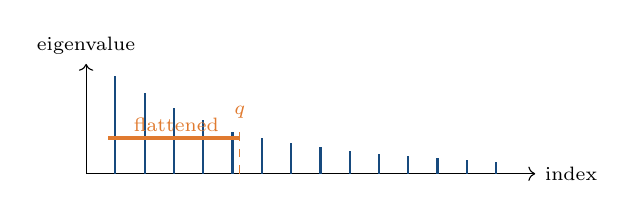
\begin{tikzpicture}[x=0.62cm,y=0.62cm]
\draw[->] (0,0) -- (9.2,0) node[right,font=\scriptsize] {index};
\draw[->] (0,0) -- (0,2.25) node[above,font=\scriptsize] {eigenvalue};
\foreach \x/\y in {0.6/2.0,1.2/1.65,1.8/1.35,2.4/1.1,3.0/0.86,3.6/0.73,4.2/0.62,4.8/0.54,5.4/0.47,6.0/0.41,6.6/0.36,7.2/0.32,7.8/0.28,8.4/0.25}
  \draw[MainBlue,thick] (\x,0) -- (\x,\y);
\draw[AccentOrange,ultra thick] (0.45,0.73) -- (3.15,0.73);
\draw[dashed,AccentOrange] (3.15,0) -- (3.15,0.93) node[above,font=\scriptsize] {$q$};
\node[font=\scriptsize,AccentOrange] at (1.85,1.0) {flattened};
\end{tikzpicture}
\end{center}
\end{frame}

% 10
\begin{frame}{Why deflation works}
\begin{columns}[T,onlytextwidth]
\column{0.55\textwidth}
\begin{block}{Spectrum before and after}
If $P_q$ is built from exact eigenvectors of $\K$, then
\[
P_q\K u_i =
\begin{cases}
\lambda_{q+1} u_i, & i\le q,\\
\lambda_i u_i, & i>q.
\end{cases}
\]
The effective largest eigenvalue becomes $\lambda_{q+1}$ instead of $\lambda_1$.
\end{block}
\begin{block}{Effect on iterations}
\[
\kappa(P_q\K)\approx \frac{\lambda_{q+1}}{\lambda_N} \ll \frac{\lambda_1}{\lambda_N}.
\]
This enables larger steps and faster convergence.
\end{block}
\column{0.40\textwidth}
\begin{center}
\begin{tikzpicture}
\begin{axis}[
width=0.95\linewidth,height=0.75\linewidth,
axis lines=left,xlabel={$q$},ylabel={proxy iterations},
xmin=0,xmax=200,ymin=0,ymax=120,xtick={0,50,100,150,200},ytick={0,40,80,120}]
\addplot[MainBlue,thick,domain=0:200,samples=100]{100/(1+0.035*x)+8};
\end{axis}
\end{tikzpicture}
\end{center}
\small Increasing $q$ improves conditioning, but estimating more eigenvectors is not free.
\end{columns}
\end{frame}

% 11
\begin{frame}{Practical limitation of EigenPro for extremely large $N$}
\begin{columns}[T,onlytextwidth]
\column{0.46\textwidth}
\begin{block}{What EigenPro fixes}
\begin{itemize}
  \item Reduces effective condition number.
  \item Allows stable large-batch updates.
  \item Uses only a small top-$q$ eigensystem.
\end{itemize}
\end{block}
\column{0.50\textwidth}
\begin{block}{What remains hard}
\begin{itemize}
  \item Kernel evaluation against many centers is still expensive.
  \item Full $\K$ cannot be materialized.
  \item Top-$q$ eigensystem must be estimated from subsamples.
  \item Large $q$ can become unstable if $s/q$ is too small.
\end{itemize}
\end{block}
\end{columns}
\vspace{0.20cm}
\begin{center}
\tikz[baseline]{\node[rounded corners,fill=SoftOrange,draw=AccentOrange,inner sep=5pt,text width=.88\linewidth,align=center]{Need a fast structured operator: preconditioning should not sit on top of $\OO(N^2)$ kernel work.};}
\end{center}
\tiny EigenPro 3.0 suggests $q\approx s/10$ in large-scale runs to balance eigen-estimation stability and cost.
\end{frame}

\section{EFGP: Fourier structure for translation-invariant kernels}

% 12
\begin{frame}{Translation-invariant kernels: useful prior structure}
\begin{block}{Definition}
A kernel is translation invariant if
\[
 k(x,x')=\kappa(x-x').
\]
This encodes stationarity: correlations depend on displacement, not absolute position.
\end{block}
\begin{columns}[T,onlytextwidth]
\column{0.48\textwidth}
\begin{itemize}
  \item Common in spatial statistics and signal processing.
  \item Smoothness and length-scale are interpretable.
  \item Includes squared exponential and Mat\'ern families.
\end{itemize}
\column{0.48\textwidth}
\begin{itemize}
  \item Fourier representation is available by Bochner's theorem.
  \item For low dimension, Cartesian frequency grids are feasible.
  \item This makes FFT/NUFFT acceleration possible.
\end{itemize}
\end{columns}
\vspace{0.05cm}
\small\textit{Key point: TI kernels expose spectral structure that FFT/NUFFT can exploit.}
\end{frame}

% 13
\begin{frame}{Bochner's theorem: kernels as spectra}
\begin{columns}[T,onlytextwidth]
\column{0.50\textwidth}
\begin{block}{Fourier representation}
For positive-definite translation-invariant kernels,
\[
\kappa(t)=\int_{\R^d}\widehat\kappa(\xi)e^{2\pi i\langle \xi,t\rangle}\,d\xi,
\quad \widehat\kappa(\xi)\geq 0.
\]
\end{block}
\begin{block}{Discrete Fourier grid}
\[
\kappa(x-x')\approx
\sum_{j\in J_m}h^d\widehat\kappa(hj)e^{2\pi ih\langle j,x-x'\rangle}.
\]
\end{block}
\column{0.45\textwidth}
\begin{center}
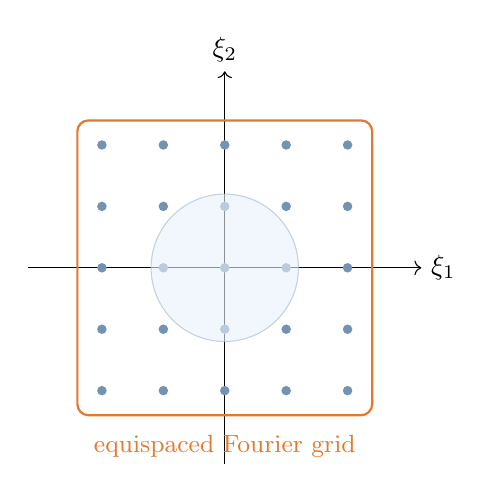
\begin{tikzpicture}[scale=0.78]
\draw[->] (-3.2,0)--(3.2,0) node[right] {$\xi_1$};
\draw[->] (0,-3.2)--(0,3.2) node[above] {$\xi_2$};
\foreach \x in {-2,-1,0,1,2}
  \foreach \y in {-2,-1,0,1,2}
    \fill[MainBlue!60] (\x,\y) circle (2.2pt);
\draw[AccentOrange,thick,rounded corners] (-2.4,-2.4) rectangle (2.4,2.4);
\node[AccentOrange,font=\small] at (0,-2.9) {equispaced Fourier grid};
\draw[MainBlue!40,fill=SoftBlue,opacity=0.6] (0,0) circle (1.2);
\end{tikzpicture}
\end{center}
\end{columns}
\end{frame}

% 14
\begin{frame}{EFGP: from kernel matrix to weight-space system}
Define basis functions
\[
\phi_j(x)=\sqrt{h^d\widehat\kappa(hj)}\, e^{2\pi i h\langle j,x\rangle},
\quad j\in J_m,
\quad M=(2m+1)^d.
\]
Then
\[
\widetilde K_{ij}=\widetilde\kappa(x_i-x_j)=\sum_{j\in J_m}\phi_j(x_i)\overline{\phi_j(x_j)}
=\PhiMat\PhiMat^*.
\]
\begin{block}{Weight-space dual system}
Instead of solving an $N\times N$ system, solve
\[
(\PhiMat^*\PhiMat+\sigma^2 I)\betaVec=\PhiMat^*\y,
\qquad \widehat f(x)=\sum_{j\in J_m}\beta_j\phi_j(x).
\]
\end{block}
\vspace{-0.1cm}
\small EFGP uses Fourier features, but not random features: the grid is deterministic and gives Toeplitz structure.
\end{frame}

% 15
\begin{frame}{Why EFGP is fast: NUFFT setup + FFT matvec}
\begin{columns}[T,onlytextwidth]
\column{0.52\textwidth}
\begin{block}{Setup}
The vector defining $\PhiMat^*\PhiMat$ and the RHS $\PhiMat^*y$ are nonuniform Fourier sums:
\[
\sum_{n=1}^{N}e^{2\pi ih\langle j,x_n\rangle},\qquad
\sum_{n=1}^{N}y_ne^{2\pi ih\langle j,x_n\rangle}.
\]
Compute with type-1 NUFFT:
\[
\OO(N+M\log M).
\]
\end{block}
\column{0.43\textwidth}
\begin{block}{Per iteration}
Because $(\PhiMat^*\PhiMat)_{j,j'}$ depends only on $j-j'$:
\[
\PhiMat^*\PhiMat v = \text{Toeplitz convolution}.
\]
Compute by padded FFT:
\[
\OO(M\log M),\quad \text{independent of } N.
\]
\end{block}
\end{columns}
\vspace{0.25cm}
\begin{center}
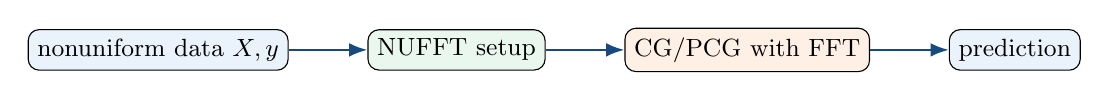
\begin{tikzpicture}[node distance=1.0cm, every node/.style={font=\small}]
\node[draw,rounded corners,fill=SoftBlue] (data) {nonuniform data $X,y$};
\node[draw,rounded corners,fill=SoftGreen,right=of data] (nufft) {NUFFT setup};
\node[draw,rounded corners,fill=SoftOrange,right=of nufft] (cg) {CG/PCG with FFT};
\node[draw,rounded corners,fill=SoftBlue,right=of cg] (pred) {prediction};
\draw[-{Latex},thick,MainBlue] (data)--(nufft);
\draw[-{Latex},thick,MainBlue] (nufft)--(cg);
\draw[-{Latex},thick,MainBlue] (cg)--(pred);
\end{tikzpicture}
\end{center}
\end{frame}

% 16
\begin{frame}{EFGP bottleneck: conditioning survives the transform}
\begin{columns}[T,onlytextwidth]
\column{0.55\textwidth}
\begin{block}{Good news}
Each iteration is cheap and does not scale with $N$.
\end{block}
\begin{block}{Bad news}
The weight-space system can still be ill-conditioned:
\[
A_W=\PhiMat^*\PhiMat+\sigma^2 I.
\]
Empirically and theoretically, condition numbers can grow near the upper-bound scale $N/\sigma^2$.
\end{block}
\column{0.40\textwidth}
\begin{center}
\begin{tikzpicture}
\begin{axis}[
width=0.95\linewidth,height=0.70\linewidth,
axis lines=left,xlabel={$\log_{10}N$},ylabel={$\log_{10}\kappa$},
xmin=1,xmax=6,ymin=0,ymax=7,xtick={1,2,3,4,5,6},ytick={0,2,4,6}]
\addplot[MainBlue,thick,mark=*] coordinates {(1,1.0) (2,2.0) (3,3.0) (4,4.05) (5,5.05) (6,6.05)};
\addplot[AccentOrange,dashed,thick] coordinates {(1,1.2) (6,6.2)};
\end{axis}
\end{tikzpicture}
\end{center}
\small Thus EFGP solves the fast-matvec problem, but not fully the iteration-count problem.
\end{columns}
\end{frame}

\section{Proposed method}

% 17
\begin{frame}{Main idea: EigenPro in frequency space}
\begin{center}
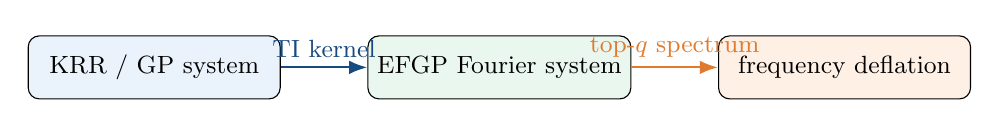
\begin{tikzpicture}[node distance=1.1cm, every node/.style={font=\small}]
\node[draw,rounded corners,fill=SoftBlue,minimum width=3.2cm,minimum height=0.8cm] (krr) {KRR / GP system};
\node[draw,rounded corners,fill=SoftGreen,minimum width=3.2cm,minimum height=0.8cm,right=of krr] (efgp) {EFGP Fourier system};
\node[draw,rounded corners,fill=SoftOrange,minimum width=3.2cm,minimum height=0.8cm,right=of efgp] (prop) {frequency deflation};
\draw[-{Latex},thick,MainBlue] (krr) -- node[above]{TI kernel} (efgp);
\draw[-{Latex},thick,AccentOrange] (efgp) -- node[above]{top-$q$ spectrum} (prop);
\end{tikzpicture}
\end{center}
\vspace{0.25cm}
\begin{block}{Hypothesis}
The dominant ill-conditioning modes of $A_W=\PhiMat^*\PhiMat+\sigma^2I$ are visible directly in the Fourier basis. Deflating them should reduce CG iterations while preserving EFGP's $\OO(N+M\log M)$ data pass.
\end{block}
\begin{block}{Core preconditioner}
Let $A_W V_q=V_q\Theta_q$ be the top-$q$ eigensystem. Define
\[
P_q=I-V_q\left(I-\theta_{q+1}\Theta_q^{-1}\right)V_q^*.
\]
Then solve $P_q A_W\beta=P_q\PhiMat^*y$ by PCG or preconditioned Richardson.
\end{block}
\end{frame}

% 18
\begin{frame}{Algorithm: Fourier-space EigenPro / preconditioned EFGP}
\small
\begin{algorithmic}[1]
\State \textbf{Input:} data $X,y$, TI kernel $\kappa$, noise/ridge $\sigma^2$, Fourier grid $(h,m)$, preconditioning level $q$.
\State Build EFGP design implicitly: $\phi_j(x)=\sqrt{h^d\widehat\kappa(hj)}e^{2\pi ih\langle j,x\rangle}$.
\State Use NUFFT to compute Toeplitz vector for $\PhiMat^*\PhiMat$ and RHS $b=\PhiMat^*y$.
\State Define fast operator $v\mapsto A_Wv=(\PhiMat^*\PhiMat+\sigma^2I)v$ using padded FFT.
\State Estimate top-$q$ eigenpairs $(V_q,\Theta_q)$ of $A_W$ using Lanczos / randomized subspace iteration with FFT matvecs.
\State Construct deflation preconditioner $P_q=I-V_q(I-\theta_{q+1}\Theta_q^{-1})V_q^*$.
\State Solve $P_qA_W\beta=P_qb$ to tolerance $\rho$.
\State Predict $\widehat f(x)=\sum_j\beta_j\phi_j(x)$ with type-2 NUFFT.
\end{algorithmic}
\vspace{0.15cm}
\begin{center}
\tikz[baseline]{\node[rounded corners,fill=SoftGreen,draw=DarkGreen,inner sep=5pt]{All expensive linear algebra uses implicit FFT/NUFFT operators; no $N\times N$ matrix is formed.};}
\end{center}
\end{frame}

% 19
\begin{frame}{What changes compared with EFGP?}
\begin{columns}[T,onlytextwidth]
\column{0.48\textwidth}
\begin{block}{EFGP baseline}
\[
A_W\beta=b.
\]
CG iteration count depends on $\kappa(A_W)$.
\end{block}
\begin{itemize}
  \item Setup: $\OO(N+M\log M)$.
  \item Per iteration: $\OO(M\log M)$.
  \item Potentially many iterations.
\end{itemize}
\column{0.48\textwidth}
\begin{block}{Proposed}
\[
P_qA_W\beta=P_qb.
\]
Dominant eigen-directions are flattened.
\end{block}
\begin{itemize}
  \item Same data pass and same FFT matvec.
  \item Extra setup for top-$q$ eigensystem.
  \item Fewer iterations if $q$ captures the spectral head.
\end{itemize}
\end{columns}
\vspace{0.25cm}
\begin{block}{Total time model}
\[
T(q) \approx T_{\text{NUFFT}} + T_{\text{eig}}(q) + n_{\text{iter}}(q)\,T_{\text{FFT-matvec}}.
\]
The optimal $q$ minimizes the \emph{sum}, not just the iteration count.
\end{block}
\end{frame}

% 20
\begin{frame}{Complexity comparison}
\small
\begin{center}
\begin{tabular}{p{0.24\linewidth}p{0.22\linewidth}p{0.22\linewidth}p{0.22\linewidth}}
\toprule
Method & Memory & Setup & Per iteration / solve \\
\midrule
Full KRR direct & $\OO(N^2)$ & $\OO(N^2)$ & $\OO(N^3)$ direct \\
CG on dense $K$ & $\OO(N)$ to $\OO(N^2)$ & kernel access & $\OO(N^2)$ matvec \\
EigenPro & no full $K$ & top-$q$ on subsample & mini-batch kernel evals \\
EFGP & $\OO(M)$ & $\OO(N+M\log M)$ & $\OO(M\log M)$ \\
Proposed & $\OO(M+Mq)$ & $\OO(N+M\log M)+T_{eig}(q)$ & fewer $\OO(M\log M)$ iterations \\
\bottomrule
\end{tabular}
\end{center}
\vspace{0.2cm}
\begin{block}{When this should help}
\begin{itemize}
  \item $d$ is small enough that $M=(2m+1)^d$ is manageable.
  \item $N$ is very large, so avoiding $\OO(N^2)$ is essential.
  \item EFGP's CG iteration count dominates after NUFFT setup.
\end{itemize}
\end{block}
\end{frame}

% 21
\begin{frame}{Top-$q$ tradeoff: too small vs too large}
\begin{columns}[T,onlytextwidth]
\column{0.50\textwidth}
\begin{block}{Small $q$}
\begin{itemize}
  \item Cheap eigen-estimation.
  \item Stable eigenpairs.
  \item But insufficient spectral flattening.
  \item More PCG iterations remain.
\end{itemize}
\end{block}
\begin{block}{Large $q$}
\begin{itemize}
  \item Stronger conditioning improvement.
  \item But eigen-estimation is expensive.
  \item Eigenvalues near the tail are harder to estimate accurately.
\end{itemize}
\end{block}
\column{0.46\textwidth}
\begin{center}
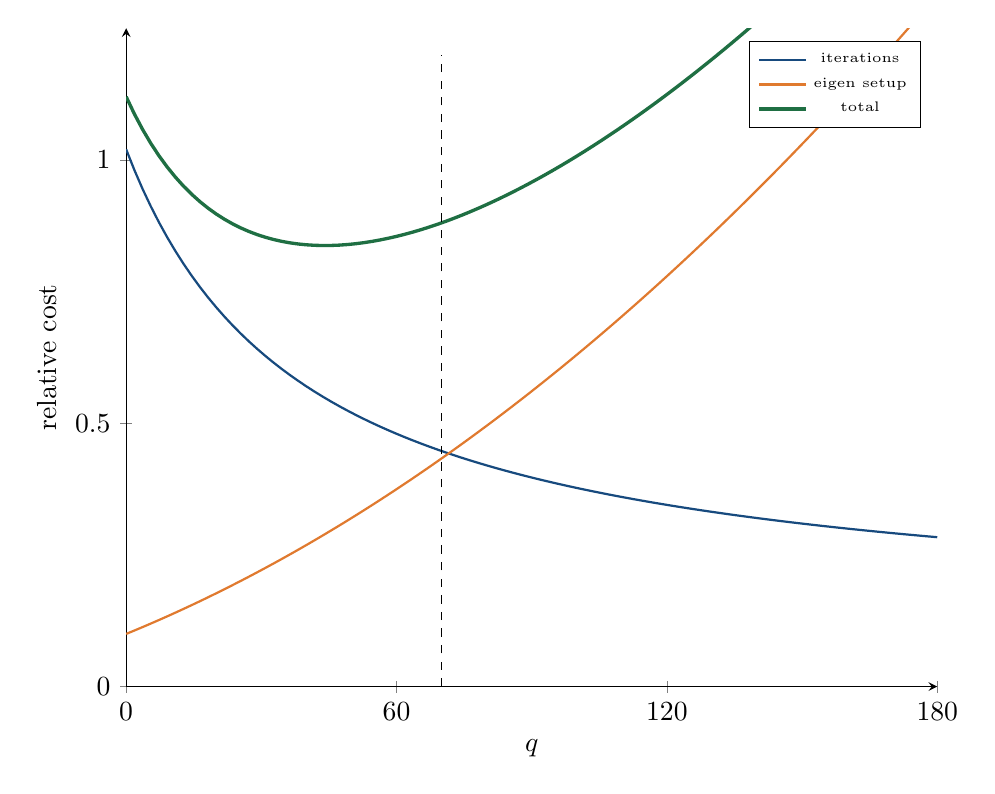
\begin{tikzpicture}
\begin{axis}[
width=0.98\linewidth,height=0.82\linewidth,
axis lines=left,xlabel={$q$},ylabel={relative cost},
xmin=0,xmax=180,ymin=0,ymax=1.25,xtick={0,60,120,180},ytick={0,0.5,1.0},legend style={font=\tiny,at={(0.98,0.98)},anchor=north east}]
\addplot[MainBlue,thick,domain=0:180,samples=100]{0.9/(1+0.025*x)+0.12};
\addlegendentry{iterations}
\addplot[AccentOrange,thick,domain=0:180,samples=100]{0.10+0.0035*x+0.000018*x*x};
\addlegendentry{eigen setup}
\addplot[DarkGreen,very thick,domain=0:180,samples=100]{0.9/(1+0.025*x)+0.12 + 0.10+0.0035*x+0.000018*x*x};
\addlegendentry{total}
\draw[dashed] (axis cs:70,0) -- (axis cs:70,1.2);
\end{axis}
\end{tikzpicture}
\end{center}
\small The experimental goal is to locate the U-shaped optimum in total runtime.
\end{columns}
\end{frame}

\section{Experiments}

% 22
\begin{frame}{Experimental protocol}
\begin{columns}[T,onlytextwidth]
\column{0.50\textwidth}
\begin{block}{Questions}
\begin{enumerate}
  \item Does preconditioning reduce iterations?
  \item Does the saved iteration time exceed eigen-setup time?
  \item How does the best $q$ change with $N$, $M$, $\sigma^2$, and kernel smoothness?
\end{enumerate}
\end{block}
\column{0.46\textwidth}
\begin{block}{Suggested datasets}
\begin{itemize}
  \item Synthetic 1D/2D regression with known truth.
  \item SE and Mat\'ern kernels.
  \item Increasing $N$: $10^4,10^5,10^6,\ldots$
  \item Fixed tolerance $\rho$ and target RMSE/EEPM.
\end{itemize}
\end{block}
\end{columns}
\vspace{0.25cm}
\begin{block}{Metrics}
\begin{itemize}
  \item CG/PCG iterations; wall-clock time; preprocessing time.
  \item Validation RMSE; posterior-mean error if reference is available.
  \item Memory footprint and sensitivity to $q$.
\end{itemize}
\end{block}
\end{frame}

% 23
\begin{frame}{Result pattern 1: convergence versus $q$}
\begin{columns}[T,onlytextwidth]
\column{0.56\textwidth}
\begin{center}
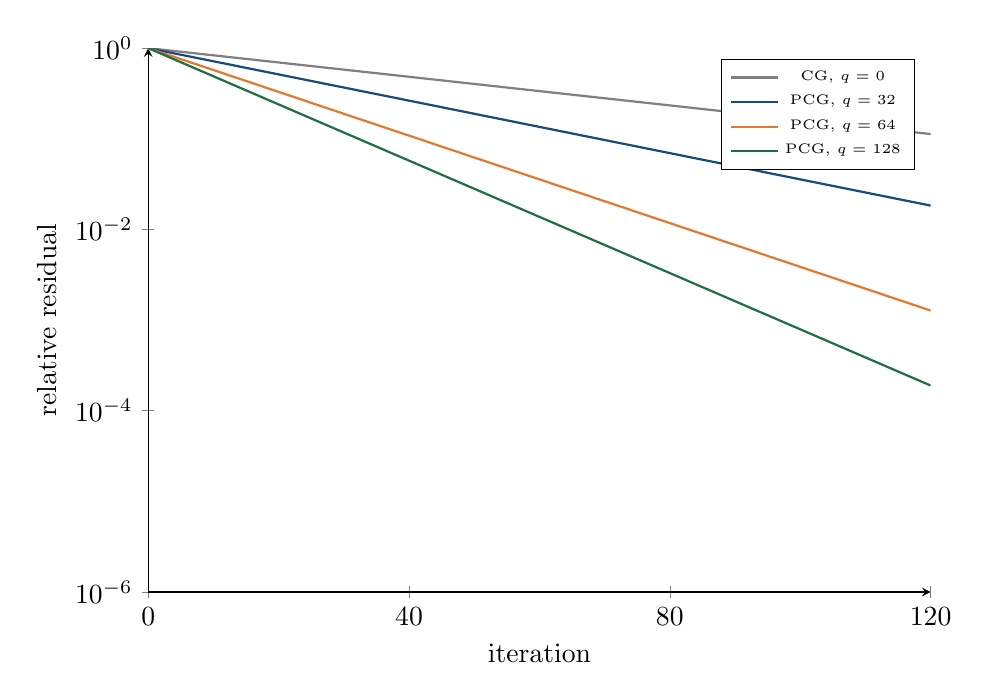
\begin{tikzpicture}
\begin{axis}[
width=0.95\linewidth,height=0.70\linewidth,
axis lines=left,xlabel={iteration},ylabel={relative residual},
ymode=log,xmin=0,xmax=120,ymin=1e-6,ymax=1,
legend style={font=\tiny,at={(0.98,0.98)},anchor=north east},
xtick={0,40,80,120},ytick={1,1e-2,1e-4,1e-6}]
\addplot[gray,thick,domain=0:120,samples=100]{exp(-x/55)};
\addlegendentry{CG, $q=0$}
\addplot[MainBlue,thick,domain=0:120,samples=100]{exp(-x/30)};
\addlegendentry{PCG, $q=32$}
\addplot[AccentOrange,thick,domain=0:120,samples=100]{exp(-x/18)};
\addlegendentry{PCG, $q=64$}
\addplot[DarkGreen,thick,domain=0:120,samples=100]{exp(-x/14)};
\addlegendentry{PCG, $q=128$}
\end{axis}
\end{tikzpicture}
\end{center}
\column{0.40\textwidth}
\begin{block}{Expected observation}
\begin{itemize}
  \item Residual decreases faster as $q$ increases.
  \item Gains saturate once dominant spectral mass is deflated.
  \item Very large $q$ may no longer improve wall-clock time.
\end{itemize}
\end{block}
\vspace{0.2cm}
\tiny This figure is a schematic trend plot; replace with logged residual curves from final runs.
\end{columns}
\end{frame}

% 24
\begin{frame}{Result pattern 2: wall-clock tradeoff}
\begin{columns}[T,onlytextwidth]
\column{0.50\textwidth}
\begin{center}
\begin{tikzpicture}
\begin{axis}[
width=0.95\linewidth,height=0.75\linewidth,
axis lines=left,xlabel={$q$},ylabel={time (normalized)},
xmin=0,xmax=160,ymin=0,ymax=1.4,xtick={0,40,80,120,160},legend style={font=\tiny,at={(0.98,0.98)},anchor=north east}]
\addplot[MainBlue,thick,mark=*] coordinates {(0,1.0) (16,0.72) (32,0.55) (64,0.42) (96,0.39) (128,0.43) (160,0.52)};
\addlegendentry{total}
\addplot[AccentOrange,dashed,thick,mark=square*] coordinates {(0,0.0) (16,0.08) (32,0.14) (64,0.24) (96,0.34) (128,0.47) (160,0.63)};
\addlegendentry{eigen setup}
\end{axis}
\end{tikzpicture}
\end{center}
\column{0.46\textwidth}
\begin{block}{Interpretation}
\begin{itemize}
  \item $q=0$ is standard EFGP-CG.
  \item Moderate $q$ can reduce total runtime.
  \item Optimal $q$ is an engineering/statistical hyperparameter.
  \item The balance depends on $M$, tolerance, and spectral decay.
\end{itemize}
\end{block}
\vspace{0.15cm}
\tiny This slide is intended for your measured runtime table. Keep the U-shape explanation even if the exact optimum changes.
\end{columns}
\end{frame}

% 25
\begin{frame}{Ablation plan: where speedups should come from}
\small
\begin{center}
\begin{tabular}{p{0.24\linewidth}p{0.32\linewidth}p{0.30\linewidth}}
\toprule
Ablation & What it tests & Expected result \\
\midrule
CG vs PCG & effect of deflation & fewer iterations \\
$q$ sweep & speed--accuracy--setup tradeoff & U-shaped total time \\
SE vs Mat\'ern & spectral decay / grid size & Mat\'ern is harder \\
small vs large $\sigma^2$ & conditioning & larger gain for small noise \\
vary $N$ at fixed $M$ & data-size dependence & NUFFT grows with $N$; iteration trend visible \\
\bottomrule
\end{tabular}
\end{center}
\vspace{0.16cm}
\begin{block}{Failure modes to report}
\begin{itemize}
  \item Top-$q$ estimation may dominate runtime when $q$ is too large.
  \item Eigenvectors become less stable when spectral gaps are small.
  \item Fourier grids do not scale well with large dimension $d$.
\end{itemize}
\end{block}
\end{frame}

\begin{frame}{Current contribution}
\begin{block}{Technical contribution}
\begin{itemize}
  \item Reformulate large-scale KRR for TI kernels in EFGP weight space.
  \item Introduce an EigenPro-style top-$q$ deflation preconditioner for the Fourier system.
  \item Implement all linear algebra through NUFFT/FFT implicit operators.
\end{itemize}
\end{block}
\begin{block}{Conceptual contribution}
\begin{itemize}
  \item EigenPro solves a \emph{spectrum} problem; EFGP solves a \emph{fast matvec} problem.
  \item Combining them targets the two main barriers simultaneously.
  \item The top-$q$ tradeoff gives a concrete, measurable knob for scalability.
\end{itemize}
\end{block}
\begin{center}
\tikz[baseline]{\node[rounded corners,fill=SoftGreen,draw=DarkGreen,inner sep=6pt]{Main message: faster iterations without returning to dense $N\times N$ computation.};}
\end{center}
\end{frame}

% 27
\begin{frame}{Next steps before final defense}
\begin{columns}[T,onlytextwidth]
\column{0.48\textwidth}
\begin{block}{Experiments to finalize}
\begin{itemize}
  \item Replace schematic curves with measured logs.
  \item Report $q$-sweep for time, iterations, and accuracy.
  \item Compare against EFGP-CG baseline at fixed tolerance.
  \item Include at least one large-$N$ case where dense methods are impossible.
\end{itemize}
\end{block}
\column{0.48\textwidth}
\begin{block}{Analysis to emphasize}
\begin{itemize}
  \item Preconditioned spectrum of $P_qA_W$.
  \item Accuracy impact of approximate eigenpairs.
  \item Runtime model: when the method helps and when it does not.
  \item Dimension limitation: $M=(2m+1)^d$.
\end{itemize}
\end{block}
\end{columns}
\vspace{0.25cm}
\begin{center}
\Large Thank you!
\end{center}
\end{frame}

\appendix

% 28
\begin{frame}{Backup: formulas for common TI kernels}
\small
\begin{columns}[T,onlytextwidth]
\column{0.48\textwidth}
\begin{block}{Squared exponential}
\[
\kappa(t)=\exp\left(-\frac{\norm{t}^2}{2\ell^2}\right),
\quad
\widehat\kappa(\xi)=(\sqrt{2\pi}\ell)^d e^{-2\pi^2\ell^2\norm{\xi}^2}.
\]
Smooth kernel $\Rightarrow$ fast spectral decay.
\end{block}
\column{0.48\textwidth}
\begin{block}{Mat\'ern}
\[
\kappa_{\nu,\ell}(t)=\frac{2^{1-\nu}}{\Gamma(\nu)}\left(\sqrt{2\nu}\frac{\norm{t}}{\ell}\right)^\nu K_\nu\left(\sqrt{2\nu}\frac{\norm{t}}{\ell}\right).
\]
Finite smoothness $\Rightarrow$ slower algebraic spectral decay.
\end{block}
\end{columns}
\vspace{0.2cm}
\begin{block}{Implication for this thesis}
Preconditioning is especially important when the Fourier system is large and ill-conditioned: low noise, large $N$, and/or slow spectral decay.
\end{block}
\end{frame}

% 29
\begin{frame}{Backup: EFGP approximation error decomposition}
\small
For a discrete Fourier grid $J_m=\{-m,\ldots,m\}^d$,
\[
\widetilde\kappa(t)-\kappa(t)=
-\sum_{n\in\mathbb{Z}^d,\,n\ne0}\kappa\left(t+\frac{n}{h}\right)
+ h^d\sum_{j\in\mathbb{Z}^d,\,j\notin J_m}\widehat\kappa(hj)e^{2\pi ih\langle j,t\rangle}.
\]
\begin{columns}[T,onlytextwidth]
\column{0.48\textwidth}
\begin{block}{Aliasing error}
Controlled by grid spacing $h$: images of the physical kernel should be far away.
\end{block}
\column{0.48\textwidth}
\begin{block}{Truncation error}
Controlled by $m$: the Fourier tail outside $[-mh,mh]^d$ should be small.
\end{block}
\end{columns}
\vspace{0.25cm}
\small For SE, both terms decay very fast; for Mat\'ern, the Fourier tail is the harder part.
\end{frame}

% 30
\begin{frame}[allowframebreaks]{References}
\tiny
\begin{thebibliography}{99}
\bibitem{bach2024}
F. Bach. \emph{Learning Theory from First Principles}. MIT Press, 2024.

\bibitem{doumeche2025}
N. Doum\`eche, F. Bach, G. Biau, and C. Boyer. \emph{Fast Kernel Methods: Sobolev, Physics-Informed, and Additive Models}. arXiv:2509.02649, 2025.

\bibitem{greengard2023}
P. Greengard, M. Rachh, and A. Barnett. \emph{Equispaced Fourier representations for efficient Gaussian process regression from a billion data points}. arXiv:2210.10210, 2023.

\bibitem{barnett2023}
A. Barnett, P. Greengard, and M. Rachh. \emph{Uniform approximation of common Gaussian process kernels using equispaced Fourier grids}. arXiv:2305.11065, 2023.

\bibitem{eigenpro3}
A. Abedsoltan, M. Belkin, and P. Pandit. \emph{Toward Large Kernel Models}. ICML, 2023.

\bibitem{ma2017}
S. Ma and M. Belkin. \emph{Diving into the shallows: a computational perspective on large-scale shallow learning}. NeurIPS, 2017.

\bibitem{ma2019}
S. Ma and M. Belkin. \emph{Kernel machines that adapt to GPUs for effective large batch training}. MLSys, 2019.

\bibitem{wilson2015}
A. G. Wilson and H. Nickisch. \emph{Kernel interpolation for scalable structured Gaussian processes}. ICML, 2015.

\bibitem{rahimi2007}
A. Rahimi and B. Recht. \emph{Random features for large-scale kernel machines}. NeurIPS, 2007.
\end{thebibliography}
\end{frame}

\end{document}
